\begin{frame}
  \begin{block}{Contexto}
    \begin{itemize}
      \item Crescimento explosivo de comunicações sem fio
      \begin{itemize}
        \item Redes ubíquas
        \item Em Dez/2011 Brasil possuía $~242.2$ milhões de telefones
        celulares ($~123,87/100$ habitantes)
      \end{itemize}
      \item Neste contexto, as \textit{\alert{Femtocells}} podem ser utilizadas
      para melhorar os serviços de voz %em uma área de cobertura limitada
    \end{itemize}
  \end{block}
  \begin{figure}[h]
  	\begin{center}
      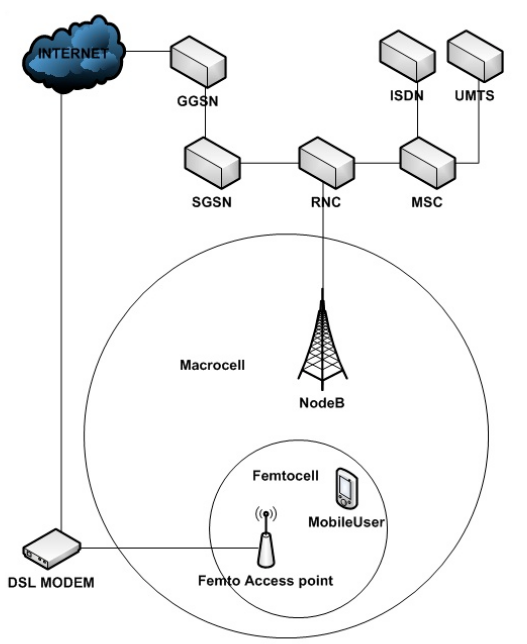
\includegraphics [scale=0.18]{./Figures/FemtocellTopology}
      \caption {Cenário Típico de utilização de \textit{Famtomcells}
      \cite{green-markov}.}
  		\label{fig:FemtocellTopology}
  	\end{center}
  \end{figure}
\end{frame}

\begin{frame}
  \begin{block}{Desafios}
    \begin{enumerate}
      \pause
      \item \alert{Escalonamento em cenários Macro-femtocell}
        \begin{itemize}
          %\item Múltiplas \textit{femtocell} vs \textit{macro-cell},
          %tipicamente co-canal
          \item Tipicamente \textit{femtocells} e \textit{macro-cell} utilizam
          o mesmo espectro (co-canal)
          \item Balanceamento de carga (concentração inadequada de clientes em
          algumas \textit{femtoncells}
        \end{itemize}
      \pause
      \item \alert{Aspectos de qualidade}
        \begin{itemize}
          \item Consumo de bateria de clientes
          \item Requisitos de QoS devem direcionar a escolha da conexão
        \end{itemize}
      \pause
      \item \alert{Consumo eficiente de energia}
        \begin{itemize}
          \item Efeito estufa
          \item Estima-se que $~57\%$ do consumo de energia em sistemas de TIC
          são gerados por clientes e dispositivos de redes móveis
        \end{itemize}
    \end{enumerate}
  \end{block}
\end{frame}

\begin{frame}
  \begin{block}{Proposta}
    \begin{itemize}
      \item \alert{Alocação ótima} de usuários em redes \textit{macro-femto}
      co-canais, permitindo \alert{auto-configuração}, com o objetivo de
      \alert{maximizar a qualidade de serviço} para as aplicações, e
      proporcionar um \alert{consumo eficiente} de energia.
    \end{itemize}
  \end{block}
\end{frame}

%\begin{frame}
%  \begin{block}{}
%    \begin{itemize}
%      \item
%    \end{itemize}
%  \end{block}
%\end{frame}

%\begin{frame}
%  \begin{block}{}
%  \end{block}
%\end{frame}

%\begin{frame}
%  \begin{figure}[h]
%  	\begin{center}
%      \includegraphics [scale=0.3]{./Figures/Device-Estimates}
%     % \caption {Estimativa de dispositivos conectados à Internet.}
%  		%\label{fig:arq-imuno}
%  	\end{center}
%  \end{figure}
%\end{frame}

%\begin{frame}{Redes de Acesso}
%	\begin{figure}[!htb]
%		\centering
%		\subfloat[DSL]{
%			\includegraphics[height=3.5cm]{./Figures/DSLaccess}
%			\label{figdroopy}}
%		\quad %espaco separador
%		\subfloat[Cable]{
%			\includegraphics[height=3.5cm]{./Figures/CableAccess}
%			\label{figsnoop}}
%		%\caption{Subfiguras}
%		%\label{fig01}
%	\end{figure}
%\end{frame}

%\begin{frame}[fragile]
%\scriptsize
%\begin{verbatim}
%\end{verbatim}
%\end{frame}
